\chapter{Sistemi di telecomunicazione su canale passa basso}
\section{Introduzione}
Obiettivo del sistema di trasmissione è di far giungere l'informazione codificata in un segnale al destinatario. Le apparecchiature di trasmissione $T_X$ e ricezione $R_X$ sono necessarie per adattare e recuperare il segnale trasmesso tenendo conto delle caratteristiche del canale: si ha attenuazione $\alpha(f)$ funzione delle frequenza e una temperatura equivalente di rumore $T_0$ che quantifica l'entità del segnale di disturbo di varia natura che si sovrappone inevitabilmente al segnale trasmesso.

\`{E} necessario quindi determinare la potenza del segnale trasmesso $P_T$ necessaria per ottenere al ricevitore un sufficiente rapporto tra la potenza attenuata del segnale ricevuto $P_R$ e la potenza media del rumore usualmente di tipo termico gaussiano bianco.
\begin{figure}[h!]
	\centering
	\begin{tikzpicture}[node distance=2cm,>=latex',thick];
	\node [block](tx) {$T_X$};
	\node [block,right of=tx,minimum height=1em,node distance=3cm](c) {$\alpha, T_0$} edge[<-](tx);
	\node [sum,right of=c](s) {$+$} edge[<-](c);
	\node [above of=s,node distance=1.5cm](n) {$h_n$} edge[->](s);
	\node [block,right of=s](rx) {$R_X$} edge[<-](s);
	\node [left of=tx](s1) {$s(t)$} edge[->](tx);
	\node [right of=rx](s2) {$\hat{s}(t)$}edge[<-](rx);
	\draw [section={$P_R$}] (s)--(rx);
	\draw [dot=$O$] (s)--(rx);
	\draw [section={$P_T$}] (tx)--(c);	
	\end{tikzpicture}
	\caption{Schema sistema di telecomunicazione su canale passa basso ad onde convogliate}
	\label{fig:sistema_trasmissione_passa_basso}
\end{figure}

La potenza del segnale in ricezione:
\begin{equation}
P_R=\frac{P_T}{\alpha} \qquad \restrict{P_R}{\text{dBm}}=\restrict{P_T}{\text{dBm}}-\restrict{\alpha}{\text{dB}}
\end{equation}

La potenza del rumore in ricezione:
\begin{equation}
P_N=k T_0 B \quad\footnotemark
\end{equation}
\footnotetext{$B$ banda monolatera del segnale}

Rapporto segnale rumore in ingresso al ricevitore:
\begin{equation}
\restrict{\frac{S}{N}}{o}=\frac{P_R}{P_N}=\frac{P_T}{\alpha k T_0 B}
\end{equation}

Rapporto segnale rumore alla uscita dal ricevitore, corretto dal fattore di rumore $F$ del ricevitore:
\begin{equation}
\restrict{\frac{S}{N}}{u}=\frac{P_R}{P_N}=\frac{P_T / \alpha}{F k T_0 B}
\end{equation}

Si dimostra che trasmettendo su due canali di trasmissione in parallelo non si può ottenere una migliore efficienza:
\begin{figure}[h!]
	\centering
	\resizebox{\textwidth}{!}{
		\begin{tikzpicture}[node distance=2cm,>=latex',thick];
		% canale superiore
		\node [block](tx) {$T_X$};
		\node [block,right of=tx,minimum height=1em,node distance=3cm](c) {$\alpha, T_0$} edge[<-](tx);
		\node [sum,right of=c](s1) {$+$} edge[<-](c);
		\node [above of=s,node distance=1.5cm](n) {$h_n$} edge[->](s1);
		\node [block,right=1.3cm of s1](rx) {$R_X$} edge[<-](s1);
		\draw [dot={$o$}] (s1)--(rx);
		\draw [section={$P_R$}] (s1)--(rx);
		\draw [section={$P_T$}] (tx)--(c);
		% canale inferiore
		\coordinate[below=1cm of tx](c0);
		\node [block,below=1cm of c0](tx2) {$T_X$};
		\coordinate[left=1.5cm of c0](c1);
		\node [left of=c1](i) {$s(t)$};
		\draw [->] (i)--(c1)|-(tx);
		\draw [->] (i)--(c1)|-(tx2);		
		\node [block,right of=tx2,minimum height=1em,node distance=3cm](c2) {$\alpha, T_0$} edge[<-](tx2);
		\node [sum,right of=c2](s21) {$+$} edge[<-](c2);
		\node [above of=s21,node distance=1.5cm](n2) {$h_n$} edge[->](s21);
		\coordinate[below=1cm of rx](c4);
		\node[sum,right=1.5cm of c4](s3){$+$};
		\node [block,right=1.3cm of s21](rx2) {$R_X$} edge[<-](s21);
		\node [right of=s3](o) {$s_T(t)$};
		\draw [->] (rx)-|node[above]{$\hat{s}(t)$}(s3);
		\draw [->] (rx2)-|node[below]{$\hat{s}(t)$}(s3);
		\draw [->](s3)--(o);		
		\draw [dot={$o$}] (s21)--(rx2);
		\draw [section={$P_R$}] (s21)--(rx2);
		\draw [section={$P_T$}] (tx2)--(c2);
		\draw [dot={$u$}] (s3)--(o);	
		\end{tikzpicture}
	}
	\caption{Schema sistema di telecomunicazione su doppio canale passa basso ad onde convogliate}
	\label{fig:sistema_trasmissione_passa_basso_doppio_canale}
\end{figure}

In uscita si ha il segnale $s_T(t)=\hat{s}_1(t)+\hat{s}_2(t)$ che ha una potenza $P_{s_T}=4 P_R$ (raddoppiando il segnale quadrupla la potenza).

In uscita si ha la somma dei rumori dei due canali, due realizzazioni di processi aleatori gaussiani (non bianchi perché filtrati)
$n_T(t)=n_1(t)+n_2(t)$, contributi incorrelati con la medesima potenza $P_N$, che risultano in una potenza del rumore in uscita
$P_{n_T}=2 P_N$

Si ha pertanto che il rapporto segnale rumore in uscita è
\[\restrict{\frac{S}{N}}{T}=2\restrict{\frac{S}{N}}{S}\]
il doppio del singono canale, ma al costo di un raddoppio della potenza trasmessa.
Raddoppiando i costi dell'intero sistema di telecomunicazione si raddoppia il rapporto segnale rumore.

\section{Sistema di trasmissione su cavo coassiale}
Il mezzo trasmissivo del sistema di telecomunicazione con trasmissione analogica in fig.\ref{fig:sistema_trasmissione_passa_basso} ipotizza che la densità spettrale del segnale $h_s$ sia costante al variare delle frequenze nella banda monolatera di trasmissione $B$ del canale, $f\in[0,B]$.

L'ipotesi di un mezzo trasmissivo che attenua in modo uguale tutte le frequenze è ideale. I mezzi di trasmissione in materiale conduttore attenuano il segnale con legge esponenziale con la distanza e in modo crescente all'aumentare della frequenza a causa dell'\keyword[effetto pelle]{effetto pelle}
\begin{equation}
\f{\alpha}{f}=\alpha_\text{sp}\sqrt{\frac{f}{f_\text{sp}}}\;[\si{\decibel\per\kilo\meter}]
\label{eq:attenuazione_esponenziale}
\end{equation}
dove la misura dell'attenuazione $\f{\alpha}{f}$ è espressa in unità logaritmiche per kilometro in riferimento all'attenuazione $\alpha_\text{sp}$\footnote{Qualche dB per km o decine dB per km su doppino} ad una specifica frequenza $f_\text{sp}$.

\begin{esempio}
	Si consideri un cavo di lunghezza $\SI{1}{\kilo\meter}$ con attenuazione $\alpha_\text{sp}= \SI{2}{\decibel\per\kilo\meter}$ alla frequenza di $\SI{1}{\mega\hertz}$. Un sistema di trasmissione su cavo coassiale costituisce un filtro passa basso affetto da attenuazione. Supponendo uno spettro di potenza del segnale $s(t)$ costante nella banda del canale, si avrà in ricezione per l'attenuazione del canale un effetto filtro con funzione di trasferimento:
	\[ H(f)=\e{-2\f{\alpha}{f}}\]
	
\begin{figure}[!ht]
\def\ampiezza{10}
\def\alphasp{2}%db/km
\def\freqsp{440}%freq taglio
\subfloat[Densità spettrale segnale trasmesso]{
\begin{tikzpicture}% coordinates
\begin{semilogxaxis}[yscale=.7,xlabel=$f$,ytick={\ampiezza},yticklabels={$h_s$},extra x ticks={\freqsp},extra x tick labels={$B$},extra x tick style={grid=major},domain=1:1e4]
\addplot coordinates {(1,\ampiezza)(\freqsp,\ampiezza)(\freqsp,0)(10000,0)};
\end{semilogxaxis}
\end{tikzpicture}
}\quad\subfloat[Densità spettrale segnale ricevuto ($\alpha_\text{sp}=\SI{2}{\decibel/\kilo\meter}$)]{
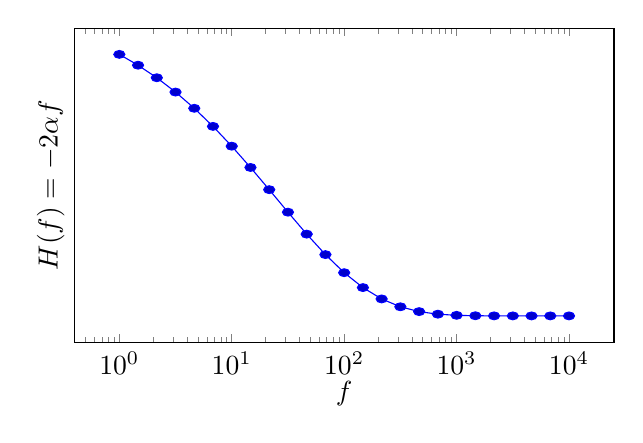
\begin{tikzpicture}% coordinates
\begin{semilogxaxis}[yscale=.7,xlabel=$f$,ylabel={$H(f)=\e{-2\f{\alpha}{f}}$},ytick={1},yticklabels={$h_s$},domain=1:1e4]
\addplot {exp(-2*\alphasp*sqrt(x/\freqsp))};
\end{semilogxaxis}
\end{tikzpicture}
}
\end{figure}
\end{esempio}

\section{Equalizzazione attiva e passiva}
Per compensare l'attenuazione del mezzo trasmissivo alle alte frequenze si può \keyword[equalizzazione]{equalizzare} in ricezione applicando un filtro con funzione di trasferimento inversa rispetto al canale:
\[\f{A}{f}=k\e{2\f{\alpha}{f}}\]
Tale equalizzazione amplifica anche il rumore, che non sarà più bianco ma avrà le componenti in alta frequenza esaltate. 

In alternativa è possibile realizzare un equalizzatore passivo che invece di amplificare lo spettro alle alte frequenze per ottenere uno spettro costante, attenui le basse frequenze, senza la necessità di una alimentazione.

L'equalizzazione viene utilizzata per segnali a banda stretta, mentre risulta problematica per segnali multiplati in frequenza.

In alternativa all'equalizzazione non lineare in ricezione si può \keyword[pre-enfasi]{pre-enfatizzare} $s(t)$ in trasmissione in modo da ottenere un segnale piatto in banda di ricezione, avendo cura di non distorcere e saturare il segnale trasmesso.

\section{Sistema di trasmissione multi-tratta}\index{sistema di trasmissione!multi-tratta}
Per compensare il fenomeno dell'attenuazione su collegamenti via cavo di grande lunghezza si progettano sistemi multi-tratta, in cui sono posti in cascata più sistemi elementari in cui si amplifica il segnale prima di trasmetterlo sulla tratta successiva.
Il sistema multi-tratta è equivalente ad un sistema con una unica tratta con densità spettrale di rumore pari alla somma delle densità spettrali di rumore incorrelate; per $m$ tratte omogenee si ha un rumore moltiplicato $m$ volte e un rapporto segnale rumore
\[\frac{S}{N}=\frac{h_s B}{\intd{0}{B}{m\cdot h_n A(f)}{f}}\]
con $B$ la banda monolatera del segnale, $h_n$ la densità spettrale di rumore in banda, $A(f)$ la curva di amplificazione di equalizzazione.
\begin{figure}[h!]
	\centering
	\subfloat[Schema sistema di telecomunicazione multi-tratta]{
		\begin{tikzpicture}[>=latex',thick,start chain=going right,node distance=5mm,every node/.style={on chain},every join/.style={->},	block/.style={draw,align=center}]
		\coordinate[join](start);
		\foreach \i in {1,...,3} {
			\node[block,join,minimum width=3em]{$\alpha$};
			\node[sum,join]{$+$};
			\begin{scope}[start branch=above, every join/.style={<-,thick,shorten <=1pt},]
				\node[on chain=going above,join]{$h_{n_\i}$};
			\end{scope}
			\node[block,join,minimum width=2em,minimum height=2em]{$A$};
			%\coordinate[right=1.3cm of s\i](m\i);
		}
		\coordinate[join](end);
		\end{tikzpicture}
	}
	
	\subfloat[Schema sistema equivalente al multi-tratta]{
		\begin{tikzpicture}[>=latex',thick,start chain=going right,node distance=5mm,every node/.style={on chain},every join/.style={->},	block/.style={draw,align=center}]
		\coordinate[join](start);
		\node[block,join,minimum width=3em]{$\alpha$};
		\node[sum,join]{$+$};
		\begin{scope}[start branch=above, every join/.style={<-,thick,shorten <=1pt}]
			\node[on chain=going above,join]{$m\cdot h_n$};
		\end{scope}
		\node[block,join,minimum width=2em,minimum height=2em]{$A$};
		\coordinate[join](end);
		\end{tikzpicture}
	}
	\caption{Schema sistema di telecomunicazione multi-tratta}
	\label{fig:sistema_trasmissione_multi_tratta}
\end{figure}

\begin{figure}[ht!]\centering
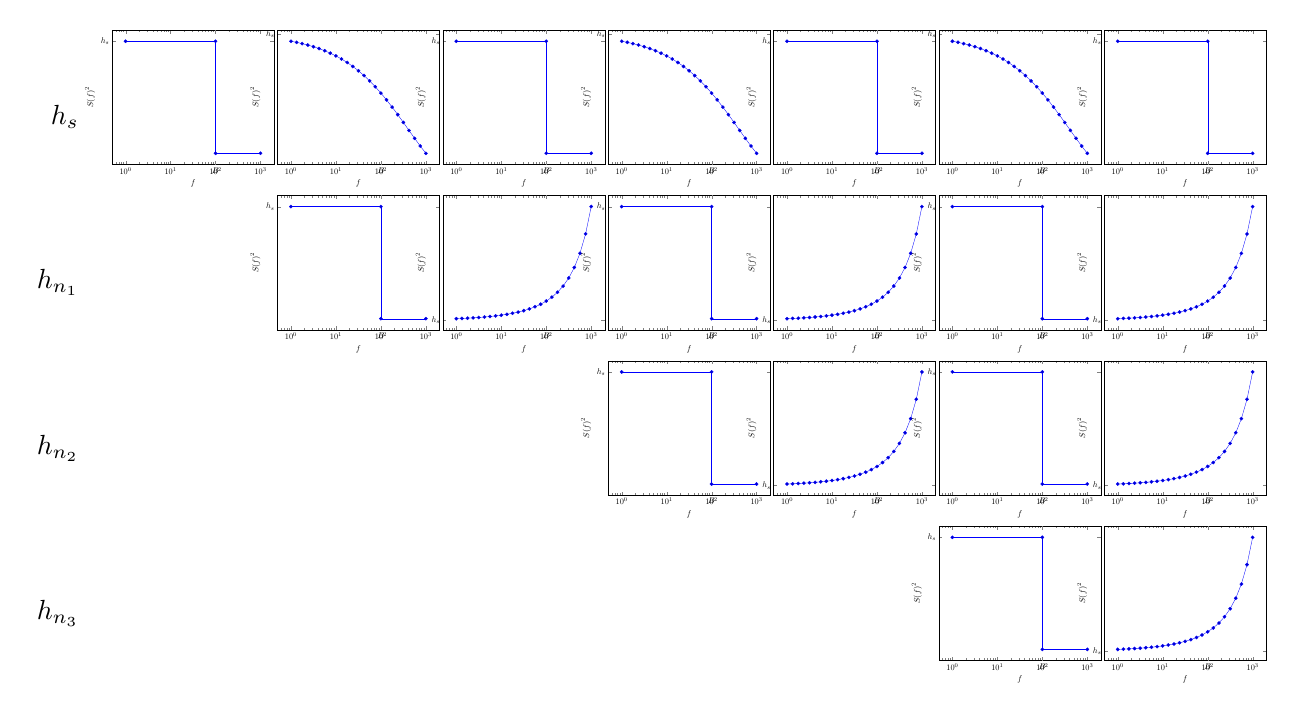
\begin{tikzpicture}[scale=.3]
\def\ampiezza{1}
\def\alphasp{1}%db/km
\def\freqsp{100}%freq taglio
\foreach \y/\s in {0/$h_s$,1/$h_{n_1}$,2/$h_{n_2}$,3/$h_{n_3}$} {
	\foreach \x in {1,...,7} {
		\ifnum \x=1\relax
		\node [left] at(-1,-\y*7+9)(n\y\x) {\s};
		\fi
		\pgfmathparse{int(\y+\y-1)}
	\def\z{\pgfmathresult}
	\ifnum\numexpr\x>\z\relax
		\begin{semilogxaxis}[black,xshift=(\x-1)*7cm,yshift=-(\y-1)*7cm,xlabel=$f$,ylabel=$\abs{S(f)}^2$,ytick={\ampiezza},yticklabels={$h_s$},extra x ticks={\freqsp},extra x tick labels={$B$},domain=1:1e3]
		\ifnum \y > 0 \relax
			\ifodd\x\relax
				\addplot {exp(.5*\alphasp*sqrt(x/\freqsp))};
			\else
				\addplot coordinates {(1,\ampiezza)(\freqsp,\ampiezza)(\freqsp,0)(\freqsp*10,0)};
			\fi
		\else
			\ifodd\x\relax
				\addplot coordinates {(1,\ampiezza)(\freqsp,\ampiezza)(\freqsp,0)(\freqsp*10,0)};
			\else
				\addplot {exp(-.5*\alphasp*sqrt(x/\freqsp))};
			\fi
		\fi
		\end{semilogxaxis}
	\fi
}}
\end{tikzpicture}
\caption{Densità spettrali di segnale e di rumore in un sistema multitratta con tratte identiche}
\end{figure}
